\documentclass{article}[18pt]
\usepackage{../../../../../format}
\lhead{Algorithms and Data Structures - Rob Powell}
\usepackage{amssymb}
\usepackage{algpseudocode}
\begin{document}
\begin{center}
\underline{\huge Recap}
\end{center}
\section{Polynomials}
\subsection{Definition}
Let $n\geqslant 0$ be an integer, and let $a_0,a_1,...,a_n$ be real numbers, $a_n\neq0$ the function:
$$f(x)=a_n\cdot x^n+a_{n-1}\cdot x^{n-1}+...+a_1\cdot x+a_0$$
is called a \textbf{polynomial}\\
\\
The numbers $a_0,...,a_n$ are called \textbf{coefficients}\\
\\
We say this is a polynomial of \textbf{degree} n\\
\\
Note: If f(x)=0, then the degree of f(x) is $-\infty$
\subsection{Types of polynomials}
\begin{tabular}{|c|c|}
	\hline 
	Degree & Name \\ 
	\hline 
	0 & constants \\ 
	\hline 
	1 & linear \\ 
	\hline 
	2 & quadratic \\ 
	\hline 
	3 & cubic \\ 
	\hline 
\end{tabular} 
\subsection{Proposition}
Let
$$f ( x ) = a _ { n } \cdot x ^ { n } + a _ { n - 1 } \cdot x ^ { n - 1 } + \ldots + a _ { 1 } \cdot x + a _ { 0 }$$
$$g ( x ) = b _ { m } \cdot x ^ { m } + b _ { m - 1 } \cdot x ^ { m - 1 } + \ldots + b _ { 1 } \cdot x + b _ { 0 }$$
be polynomials of degrees n and m respectively
\begin{itemize}
	\item the \textbf{sum} of the polynomials f(x)+g(x) is a polynomial of \textbf{degree} max\{n,m\}
	\item the \textbf{product} of the polynomials $f(x)\cdot g(x)$ is a polynomial of degree n+m. Product is multiplying two functions together
	\item the \textbf{composition} of the polynomials $f(g(x))$ is a polynomial of degree $n\cdot m$. Composition is replacing the x terms in f(x) with g(x). Remember $f(g(x))\neq g(f(x))$
	\item The degree is the important part, as most other parts are insignificant as x becomes large
\end{itemize}
\section{Positive integer powers}
\subsection{Definition}
For a positive integer n and a real number a,
$$a ^ { n } = \underbrace { a \cdot a \cdot \ldots \cdot a } _ { n }$$
The number a is called the \textbf{base} and n is called the \textbf{exponent} or the \textbf{power}
\subsection{Basic rules}
For positive integers n,m and a real number a
$$a^n\cdot a^m=a^{n+m}$$
$$(a^n)^m=a^{n\cdot m}$$
\section{Rational Powers}
\subsection{Definitions}
\subsubsection{Definition 1}
For a real number $a\neq 0$ (because $0^0$ is undefined)
$$a^0=1$$
\subsubsection{Definition 2}
For a positive integer n and a real number $a\neq 0$
$$a^{-n}=\dfrac{1}{a^n}$$
\subsubsection{Defintion 3}
For a positive integer n and a real number $a\geqslant 0$, we define $a^{\frac{1}{n}}$ as the \textbf{n-th root} of a\\
\\
That is $a^{\frac{1}{n}}$ is a real number x with the property $x^n=a$ $(a^{\frac{1}{n}}=x\Leftrightarrow x^n=a)$\\
\\
We also write $a^{\frac{1}{n}}=\sqrt[n]{a}$
\subsection{More on Rational Powers}
When $a>0$ and n is even the equation
$$x^n=a$$
may have more than one real solution\\
\\
For example, the equation 
$$x^2=4$$
has two solutions, 2 and -2\\
\\
By convention, we normally consider the \textbf{positive solution} as the value of the n-th root of a\\
\\
\\
Notice that we assumes that $a>0$\\
If n is an \textbf{odd} integer, then we can extend the definition of the n-th root to \textbf{negative} bases a because the equation
$$a^n=a$$
still has real solutions\\
For example:
$$(-8)^{\frac{1}{3}}=-2$$
because
$$(-2)^3=-8$$
\subsection{Definition}
Let m be an integer and let n be a positive integer. For a real number $a>0$,
{\Large$$a^{\frac{m}{n}}=(a^m)^\frac{1}{n}=(a^\frac{1}{n})^m$$}
$ $\\
\\
For example
{\large$$8^\frac{2}{3}=4$$
$$8^{-\frac{2}{3}}=\frac{1}{4}$$}
\section{Real Powers}
Because the set of rational numbers is a dense subset (belong in or limit points) of the real numbers we can also define real powers. That is, we can define $a^x$ for any positive real number a and any real number x.\\
\\
The formal technique to do this is by taking the \textbf{limit}.\\
\\
That means that for any real number x, we can find a rational $\frac{m}{n}$ arbitrarily close to x, so that $a^{\frac{m}{n}}$ is also arbitrarily close to $a^x$.
\section{Exponential Functions}
\subsection{Definition}
For a fixed positive real number a, the function
$$f(x)=a^x$$
is called \textbf{exponential function} with base a
\subsection{More on exponential functions}
Exponential functions are defined over the set of real number, so the above function is defined for every real number x\\
\\
Their values are positive real numbers\\
\begin{center}
	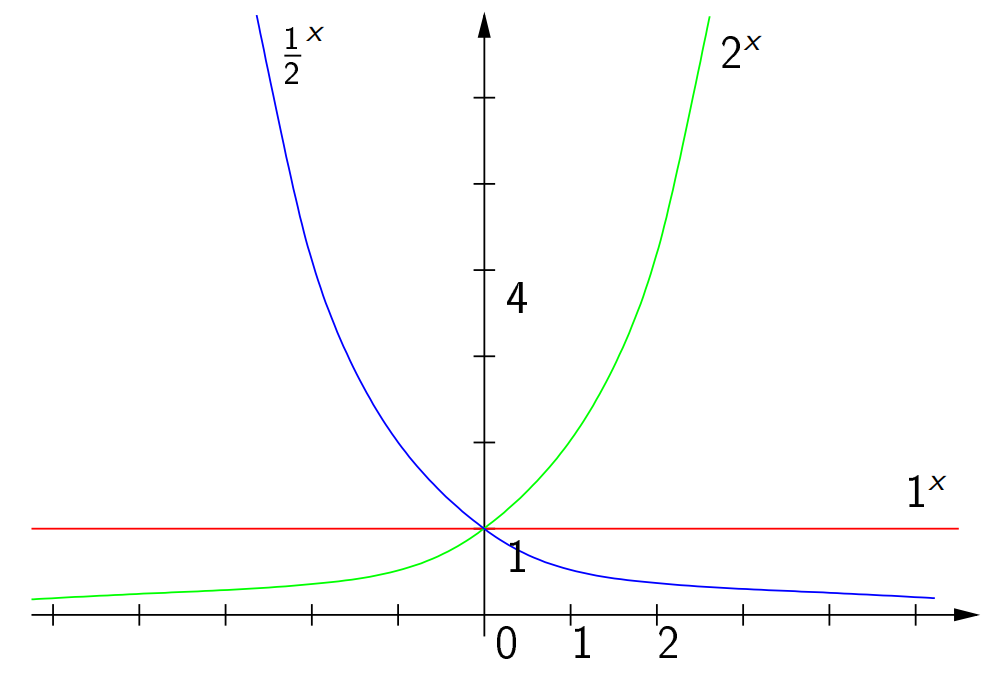
\includegraphics[scale=0.4]{exponential}
\end{center}
\begin{itemize}
	\item The exponential functions are positive everywhere
	\item At zero their value is 1
	\item For base $a>1$ the function f(x)=$a^x$ increases monotonically (never constant, never decreases, rate of increase is continually increasing). It grows fast compared to many other functions
\end{itemize}
\subsection{Proposition 1}
Let $a,b,x,y$ be real numbers with $a,b>0$. Then
\begin{itemize}
	\item $a^x\cdot a^y=a^{x+y}$
	\item $a^{-x}=\frac{1}{a_x}$
	\item $(a^x)^y=a^{x\cdot y}$
	\item $(ab)^x=a^x\cdot b^x$
\end{itemize}
\subsection{Proposition 2}
Let $a,x,y$ be real numbers with $a>1$. Then for $x\leqslant y$, $a^x\leqslant a^y$\\
\\
We say that the exponential function with $a>1$ increases \textbf{monotonically}
\section{Logarithms}
\subsection{Definition}
For real positive number $x,a$ with $a\neq 1$, the \textbf{logarithm} of x to the \textbf{base} a, written $\log_ax$ as the unique real number y that satisfies $a^y=x$\\
\\
That is, if we raise a to the power of $\log_ax$ we get x:
{\large$$a^{\log_ax}=x$$}
\subsection{Examples}
$$log_a1=0$$
$$\log_aa=1$$
$$\log_aa^2=2$$
$$\log_a\frac{1}{a}=-1$$
\subsection{Properties of logarithms}
\subsubsection{Proposition}
Let $a,x,y$ be positive real numbers $a\neq 1$ we have
\begin{itemize}
	\item $\log_axy=log_ax+log_ay$
	\item $\log_a\frac{x}{y}=\log_ax-\log_ay$
	\item $\log_ax^s=s\cdot \log_ax$ for any real s
\end{itemize}
\textbf{Proof}
{\large
\begin{itemize}
	\item $a^{\log_ax+\log_ay}=a^{\log_ax}\cdot a^{\log_ay}=x\cdot y$
	\item $a^{\log_ax-\log_ay}=a^{\log_ax}\cdot a^{-\log_ay}=\frac{x}{y}$
	\item $a^{s\log_ax}=(a^{\log_ax})^s=x^s$
\end{itemize}}
\subsubsection{Proposition}
Let $a,b,x$ be positive real numbers, $a,b \neq 1$, Then
$$\log_ax=\dfrac{log_bx}{\log_ba}$$
So logarithms to different constant bases only differ by a constant\\
\\
\textbf{Proof}\\
By the definition
{\large $$x=a^{\log_ax}$$ }
It follows that
{\large $$\log_bx=\log_ba^{\log_ax}=\log_ax\cdot\log_ba$$}
\subsubsection{Natural Logarithms}
The natural logarithm is denoted $\ln x$\\
2,e and 10 are the "special" bases in CS
\subsection{Logarithmic Function}
\subsubsection{Definition}
Let a be a positive real number $a\neq 1$. The function
$$f(x)=\log_ax$$
Defined for positive real numbers is called \textbf{logarithmic}
\begin{itemize}
	\item Logarithmic functions are \textbf{inverses} of exponential functions
	\item They are only defined on positive real numbers
	\item For any base, the logarithm of 1 to that base is 0
	\item For $a>1$ logarithms to the base a increase monotonically.
\end{itemize}



\end{document}